\documentclass[11pt]{article}

\usepackage[margin=1in]{geometry}
\usepackage[T1]{fontenc}
\usepackage{lmodern}
\usepackage{amsmath, amssymb, amsthm, bm}
\usepackage{graphicx}
\usepackage{booktabs}
\usepackage{hyperref}
\usepackage{caption}
\usepackage{subcaption}
\usepackage{float}
\usepackage{enumitem}
\usepackage{setspace}
\usepackage{xcolor}

\hypersetup{
  colorlinks=true,
  linkcolor=blue!60!black,
  citecolor=blue!60!black,
  urlcolor=blue!60!black
}

\graphicspath{{../results/}}
\setstretch{1.0}
\setlength{\parskip}{0.45em}
\setlength{\parindent}{0pt}

\title{Quantum Feature Maps as Simple Embeddings for Machine Learning}
\author{Steven Zhou\\PHYS 345 Final Project}
\date{April 26, 2026}

\begin{document}

\maketitle

\begin{abstract}
Kernel methods provide a clean way to separate the choice of representation from the choice of downstream learning algorithm. Quantum computing suggests a natural alternative representation mechanism because a small number of qubits already lives in a high-dimensional Hilbert space, and data can be encoded into this space through parameterized gates. This report studies a minimal version of that idea using one- and two-qubit feature maps implemented in Qiskit. The main question is whether such feature maps behave as meaningful embeddings, in the precise sense that state overlaps induce nonlinear similarity measures that can be used for learning. I derive the kernel generated by a one-qubit rotation map, situate this toy model within the broader quantum-kernel literature, show how a two-qubit entangling map changes the geometry of similarity, and compare quantum-kernel classification against raw-input and classical-feature baselines on a simple nonlinear dataset. The simulated one-qubit kernel agrees with the analytic prediction to relative error $1.66\times 10^{-16}$. On a two-dimensional moon dataset, logistic regression on raw inputs achieved test accuracy $0.8889$, while a support vector machine using the quantum kernel achieved $0.9444$. These results do not demonstrate quantum advantage, but they do provide a reproducible example in which quantum states act as explicit feature generators for similarity-based learning.
\end{abstract}

\section{Problem Statement and Fundamental Claim}

The central problem of this project is to understand whether a quantum circuit can be interpreted as a useful embedding map for classical data. In standard machine learning, one often takes an input vector $x$ and maps it into a larger feature space $\Phi(x)$ where the target classes become more easily separable. This can be done explicitly, by constructing additional features, or implicitly, through a kernel function that computes inner products in the transformed space without ever writing down the full feature vector. The fundamental claim explored here is that a quantum circuit naturally defines such an embedding, because the map
\begin{equation}
x \mapsto |\psi(x)\rangle = U(x)|0\rangle^{\otimes n}
\label{eq:featuremap}
\end{equation}
sends classical input data into a quantum state in a Hilbert space of dimension $2^n$. Once the data is encoded this way, the overlap between two encoded states defines a kernel
\begin{equation}
K(x,x') = |\langle \psi(x) | \psi(x') \rangle|^2,
\label{eq:kerneldef}
\end{equation}
which can be inserted into an ordinary classical kernel method such as a support vector machine (SVM).

For this project, the claim is deliberately modest. I do not attempt to show that the quantum kernel outperforms all classical kernels or that the chosen problem is beyond classical reach. Instead, I test the narrower and more teachable statement that simple quantum feature maps already produce nonlinear similarity functions with interpretable geometric structure and measurable learning value. If that statement is true, then quantum circuits can be understood not only as full computational models but also as structured feature generators.

\section{Scientific Motivation}

There are two reasons this question is scientifically interesting. The first is conceptual. A recurring theme in quantum machine learning is that quantum systems provide access to very large vector spaces with relatively few physical degrees of freedom \cite{schuld2019feature, havlicek2019feature}. Even when no computational advantage is claimed, that observation invites a useful reinterpretation of quantum states. Rather than asking a quantum computer to replace a classical learner outright, one can ask it to define a representation in which similarity is measured differently from standard Euclidean distance. This makes contact with familiar ideas from statistical learning theory while keeping the quantum role concrete and mathematically transparent.

The second motivation is methodological. Many proposed quantum machine-learning algorithms are difficult to interpret because the circuits are deep, the data encoding is opaque, and the learning rule is mixed together with the quantum dynamics. A small feature-map project avoids those complications. The encoded states are simple enough to analyze by hand, the kernel can be visualized directly, and the downstream model is a standard classical SVM whose behavior is well understood. That makes the project appropriate for a PHYS 345 audience. It isolates a genuinely new idea without requiring a large amount of additional formalism beyond the course background.

This perspective also connects naturally to the current literature. Havl\'{\i}\v{c}ek et al.\ studied feature-map circuits whose overlaps define kernels that may be difficult to estimate classically in general \cite{havlicek2019feature}. Schuld and Killoran emphasized that quantum data encoding is formally analogous to the feature-space viewpoint of classical kernels \cite{schuld2019feature}. My project occupies the pedagogically useful minimal end of this spectrum. I focus on feature maps simple enough that one can derive the kernel analytically in the one-qubit case and numerically inspect it in the two-qubit case. The value of the project therefore lies less in novelty than in clarity. It exhibits the kernel interpretation of quantum embeddings in a fully reproducible setting using Qiskit \cite{qiskitdocs, qiskitkerneldocs}.

\section{Literature Context and Scope}

Because the rubric asks for an in-depth literature review rather than an original research paper, it is important to make clear how this report relates to prior work. The present project does not claim to introduce a new quantum kernel or a new learning protocol. Instead, it distills a specific theme from the literature into a compact example that can be explained carefully from first principles.

The key conceptual source is the observation by Schuld and Killoran that quantum machine learning can be framed in the language of feature maps and kernels \cite{schuld2019feature}. Their paper makes the formal point that any quantum data encoding defines an implicit feature map into Hilbert space, and that inner products of encoded states therefore define kernels in direct analogy with classical kernel methods. That viewpoint is foundational for this report. In a sense, the one-qubit derivation below is a stripped-down classroom-scale realization of their general argument.

The work of Havl\'{\i}\v{c}ek et al.\ represents a more ambitious direction \cite{havlicek2019feature}. There the emphasis is not merely interpretive clarity but the possibility that certain quantum feature spaces may be difficult to reproduce classically. Their circuits are deeper and their claims are correspondingly stronger. My report intentionally stops short of that frontier. I do not attempt a complexity-theoretic separation, and I do not present hardware data. Instead, I ask a narrower question that is better suited to a PHYS 345 final project. Can one see, in a transparent and reproducible toy setting, how quantum circuits generate nonlinear similarity structure?

The project is therefore best understood as a pedagogical literature-based reconstruction rather than as a simplified copy of a published demo. The one-qubit rotation map and the two-qubit entangling map used here were chosen specifically for this report because they are easy to analyze and visualize. The dataset, parameter choices, and figures were generated independently in the accompanying code rather than copied from the Qiskit textbook or a published benchmark. In particular, the numerical experiments use a custom parameter set. I use $60$ points on $[0,2\pi]$ for the analytic validation, a moon dataset with $240$ samples and noise level $0.16$, and a two-qubit entangling scale $\lambda=1.5$. This matters for the rubric because it makes clear which parts of the report are my own implementation and exposition, and which parts are based on prior literature.

\section{Theory of Quantum States as Feature Embeddings}

\subsection{One-qubit encoding}

Consider a single real input $x$ encoded into one qubit by a rotation about the $y$ axis
\begin{equation}
|\psi(x)\rangle = R_y(x)|0\rangle.
\label{eq:rymap}
\end{equation}
Since
\begin{equation}
R_y(x)|0\rangle = \cos\left(\frac{x}{2}\right)|0\rangle + \sin\left(\frac{x}{2}\right)|1\rangle,
\label{eq:singlequbitstate}
\end{equation}
the overlap between two encoded inputs $x$ and $x'$ is
\begin{align}
\langle \psi(x)|\psi(x')\rangle
&=
\cos\left(\frac{x}{2}\right)\cos\left(\frac{x'}{2}\right)
\sin\left(\frac{x}{2}\right)\sin\left(\frac{x'}{2}\right) \nonumber \\
&=
\cos\left(\frac{x-x'}{2}\right),
\label{eq:onequbitoverlap}
\end{align}
where the final step uses the cosine difference identity. Therefore the quantum kernel becomes
\begin{equation}
K(x,x') = \left|\langle \psi(x)|\psi(x')\rangle\right|^2
= \cos^2\left(\frac{x-x'}{2}\right).
\label{eq:onequbitkernel}
\end{equation}

Equation~\eqref{eq:onequbitkernel} already shows the essential point. The quantum embedding converts a scalar input into a nonlinear similarity measure. Nearby points in $x$ have kernel value close to $1$, while points separated by $\pi$ become nearly orthogonal and therefore highly dissimilar. The kernel depends only on the difference $x-x'$, which makes it a translation-invariant periodic kernel. The state space here is only two-dimensional, yet it already generates a nontrivial geometry not obvious from the raw input alone.

\subsection{Why the kernel is valid}

It is important to verify that Eq.~\eqref{eq:kerneldef} defines a legitimate kernel for classical learning. For any collection of data points $\{x_i\}_{i=1}^m$, define the Gram matrix $G$ by
\begin{equation}
G_{ij} = \langle \psi(x_i)|\psi(x_j)\rangle.
\label{eq:gram}
\end{equation}
Then the kernel matrix used in this project is
\begin{equation}
K_{ij}=|G_{ij}|^2.
\label{eq:kernelgram}
\end{equation}
This matrix is positive semidefinite because it can be written as an inner product matrix in the tensor-product feature space
\begin{equation}
K_{ij}
=
\langle \psi(x_i)\otimes \psi(x_i)^* , \psi(x_j)\otimes \psi(x_j)^* \rangle.
\label{eq:tensorpsd}
\end{equation}
Hence for any coefficients $c_i$,
\begin{equation}
\sum_{i,j} c_i^* K_{ij} c_j
=
\left\| \sum_i c_i \, \psi(x_i)\otimes \psi(x_i)^* \right\|^2 \ge 0.
\label{eq:psdproof}
\end{equation}
This proves that the overlap kernel can be supplied to an SVM without violating the assumptions of the classical algorithm.

\subsection{Two-qubit entangling map}

The one-qubit example is analytically transparent but too simple to reveal the role of entanglement. To study a richer embedding, I use a two-qubit feature map for a two-dimensional input vector $\bm{x}=(x_1,x_2)$
\begin{equation}
U(\bm{x})
=
\mathrm{CX}_{01}\,
R_z\!\left(\lambda(x_1+x_2)\right)_1\,
\mathrm{CX}_{01}\,
R_y(x_1)_0 R_y(x_2)_1,
\label{eq:twoqubitmap}
\end{equation}
with entangling scale $\lambda = 1.5$ in the numerical experiments. The first pair of $R_y$ rotations encodes the two coordinates independently. The controlled-NOT and intermediate $R_z$ gate then inject a correlated phase that depends on both features. This is the simplest kind of departure from a purely factorized embedding. The state geometry is no longer determined by separate one-dimensional similarities.

The exact analytic form of the corresponding kernel is less illuminating than in the one-qubit case, so I study it numerically by constructing the statevector in Qiskit and evaluating Eq.~\eqref{eq:kerneldef} directly. What matters for the learning problem is that the entangling term changes the way pairwise similarities are distributed across the dataset. This makes the quantum kernel more expressive than a separable product of single-qubit kernels while remaining easy to reproduce.

\section{Methodology}

\subsection{Software and computational setup}

All simulations were carried out in Python using Qiskit's circuit and quantum-information tools, together with \texttt{NumPy}, \texttt{scikit-learn}, \texttt{matplotlib}, and \texttt{seaborn} \cite{qiskitdocs, qiskitkerneldocs, sklearn}. Rather than estimating overlaps by sampling measurements, I used exact statevector simulation. This was the right choice for the pedagogical goals of the project because it removes shot noise and allows the kernel structure to be seen directly.

The repository accompanying this report contains all code required to reproduce the results. The main script is \texttt{scripts/run\_experiment.py}. Running that script generates the figures and writes the quantitative outputs to \texttt{results/metrics.json}. The code is modularized into separate files for feature maps, kernels, data generation, plotting, and experiment orchestration so that each step of the analysis is transparent and easy to modify.

\subsection{Experiment 1 validating the analytic one-qubit kernel}

The first experiment checks that the Qiskit implementation reproduces Eq.~\eqref{eq:onequbitkernel}. I sampled $60$ input values evenly spaced on $[0,2\pi]$ and computed the full $60\times 60$ kernel matrix in two ways
\begin{enumerate}[label=\arabic*.]
\item analytically using Eq.~\eqref{eq:onequbitkernel}
\item numerically by constructing the statevector for each input and evaluating the overlap in Eq.~\eqref{eq:kerneldef}
\end{enumerate}

To quantify agreement, I measured the relative Frobenius error
\begin{equation}
\epsilon_{\mathrm{rel}}
=
\frac{\|K_{\mathrm{analytic}}-K_{\mathrm{simulated}}\|_F}
{\|K_{\mathrm{analytic}}\|_F}.
\label{eq:frob}
\end{equation}
This provides a direct metric for whether the code realizes the intended feature map.

\subsection{Experiment 2 classification with a two-qubit kernel}

The second experiment asks whether a simple quantum feature map can improve classification on a nonlinear toy dataset. I used the two-dimensional \texttt{make\_moons} dataset from \texttt{scikit-learn}, with $240$ samples, noise level $0.16$, and random seed $7$ \cite{sklearn}. The data were split into $70\%$ training and $30\%$ testing sets using stratified sampling. Each coordinate was then rescaled to the interval $[0,\pi]$ before being inserted into the two-qubit circuit. This scaling keeps the inputs in a natural range for rotation angles and makes the learned geometry easier to interpret.

For the classical baselines I trained
\begin{enumerate}[label=\arabic*.]
\item logistic regression on the raw two-dimensional input
\item logistic regression after a degree-$3$ polynomial feature lift
\item an SVM with the standard radial basis function (RBF) kernel.
\end{enumerate}
For the quantum model I computed the training kernel matrix
\begin{equation}
K^{\mathrm{train}}_{ij}
=
\left|\left\langle \psi(\bm{x}^{\mathrm{train}}_i)\middle|\psi(\bm{x}^{\mathrm{train}}_j)\right\rangle\right|^2
\label{eq:trainkernel}
\end{equation}
and the test matrix
\begin{equation}
K^{\mathrm{test}}_{ab}
=
\left|\left\langle \psi(\bm{x}^{\mathrm{test}}_a)\middle|\psi(\bm{x}^{\mathrm{train}}_b)\right\rangle\right|^2,
\label{eq:testkernel}
\end{equation}
then passed these matrices to an SVM with \texttt{kernel=precomputed}. Test accuracy was used as the primary performance metric.

This design compares representation choices while keeping the final classifier conventional. In particular, the quantum feature map changes the similarity notion but does not alter the SVM optimization problem itself. That clean separation is important because it lets the reader attribute any change in performance to the embedding rather than to a different learning algorithm.

\section{Results}

\subsection{Single-qubit kernel structure}

Figure~\ref{fig:onequbitheatmap} shows the full one-qubit kernel matrix obtained from the Qiskit statevector simulation. The matrix displays the banded, periodic structure predicted by Eq.~\eqref{eq:onequbitkernel}. Points with similar angles have large overlap, while points separated by approximately $\pi$ become nearly orthogonal. Figure~\ref{fig:analyticcompare} compares the simulated kernel as a function of input difference against the exact analytic expression. The two curves are visually indistinguishable.

The numerical agreement is summarized by the relative Frobenius error
\begin{equation}
\epsilon_{\mathrm{rel}} = 1.66\times 10^{-16},
\label{eq:errorvalue}
\end{equation}
which is essentially machine precision. This validates both the feature-map implementation and the interpretation of the kernel as a state overlap.

\begin{figure}[H]
\centering
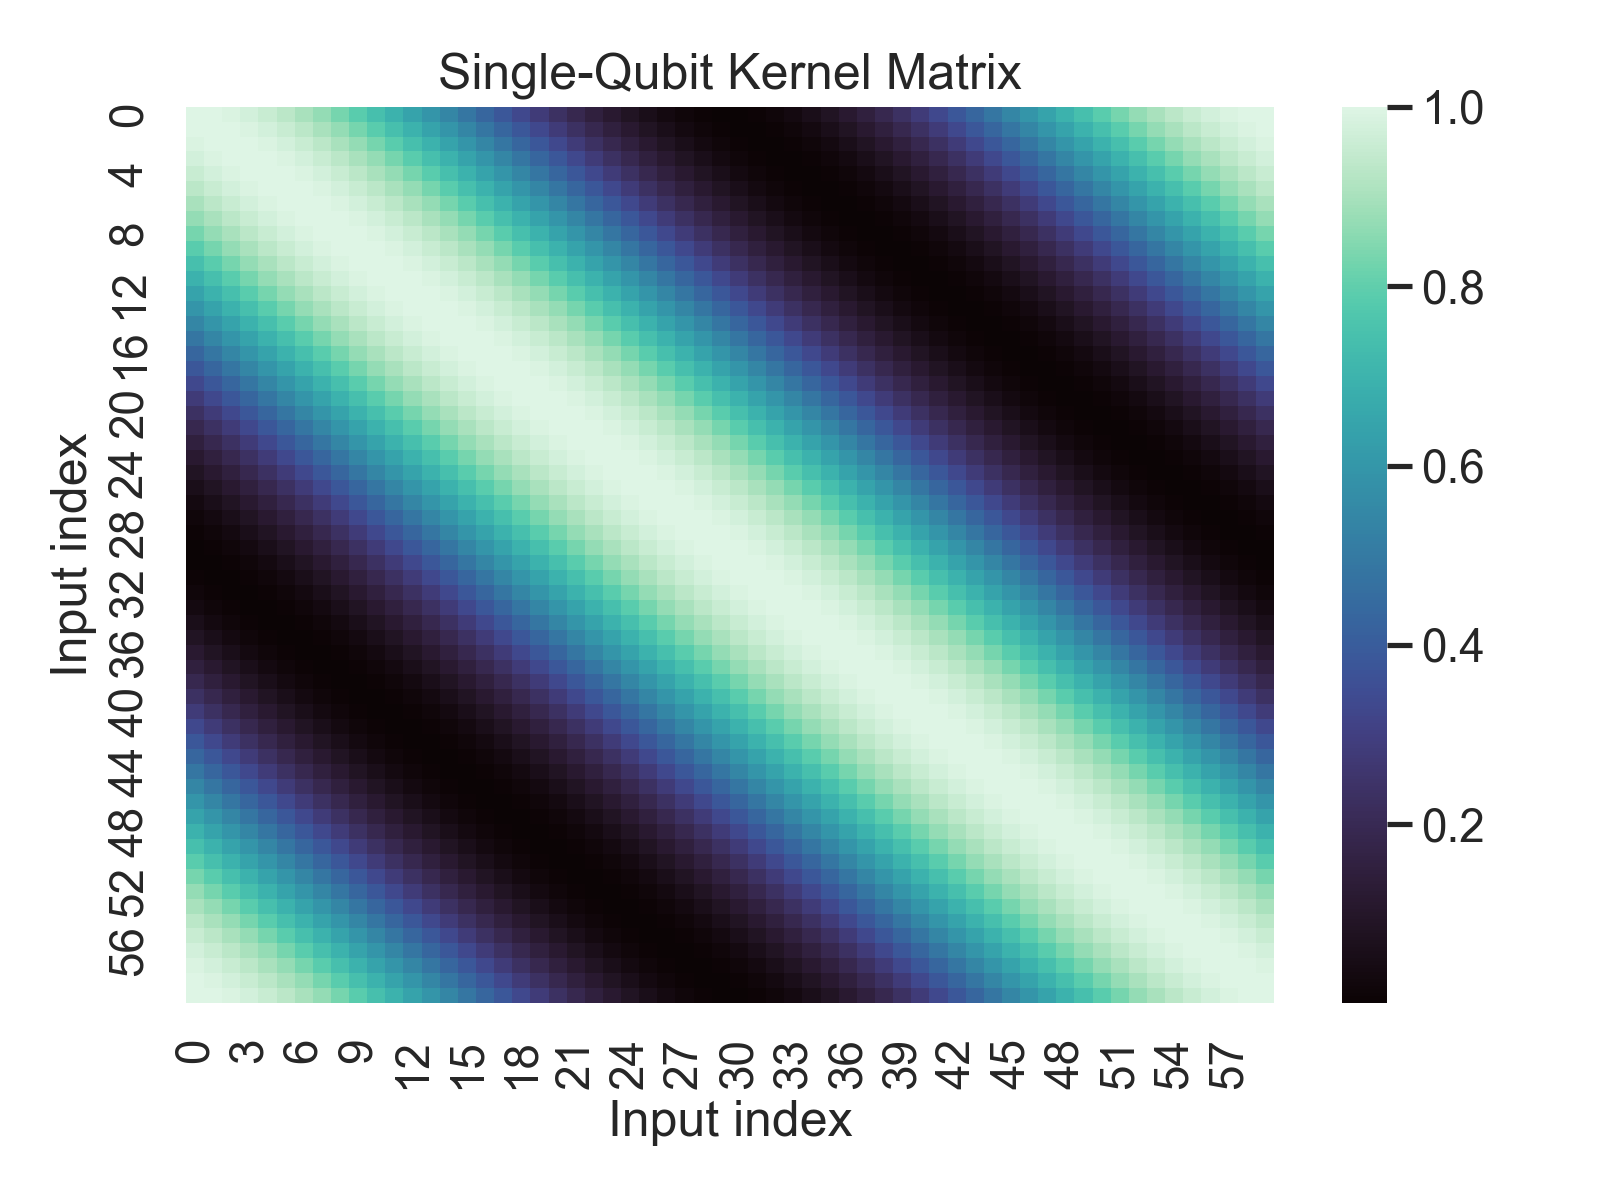
\includegraphics[width=0.72\textwidth]{one_qubit_kernel_heatmap.png}
\caption{Kernel matrix for the one-qubit feature map $|\psi(x)\rangle = R_y(x)|0\rangle$ evaluated on $60$ points in $[0,2\pi]$. The horizontal and vertical axes denote the sampled input index, ordered from $x=0$ to $x=2\pi$, and the color scale gives the kernel value $K(x_i,x_j)$. The bright diagonal and periodic bands reflect the analytic form in Eq.~\eqref{eq:onequbitkernel}. This figure was generated by the code accompanying this report.}
\label{fig:onequbitheatmap}
\end{figure}

\begin{figure}[H]
\centering
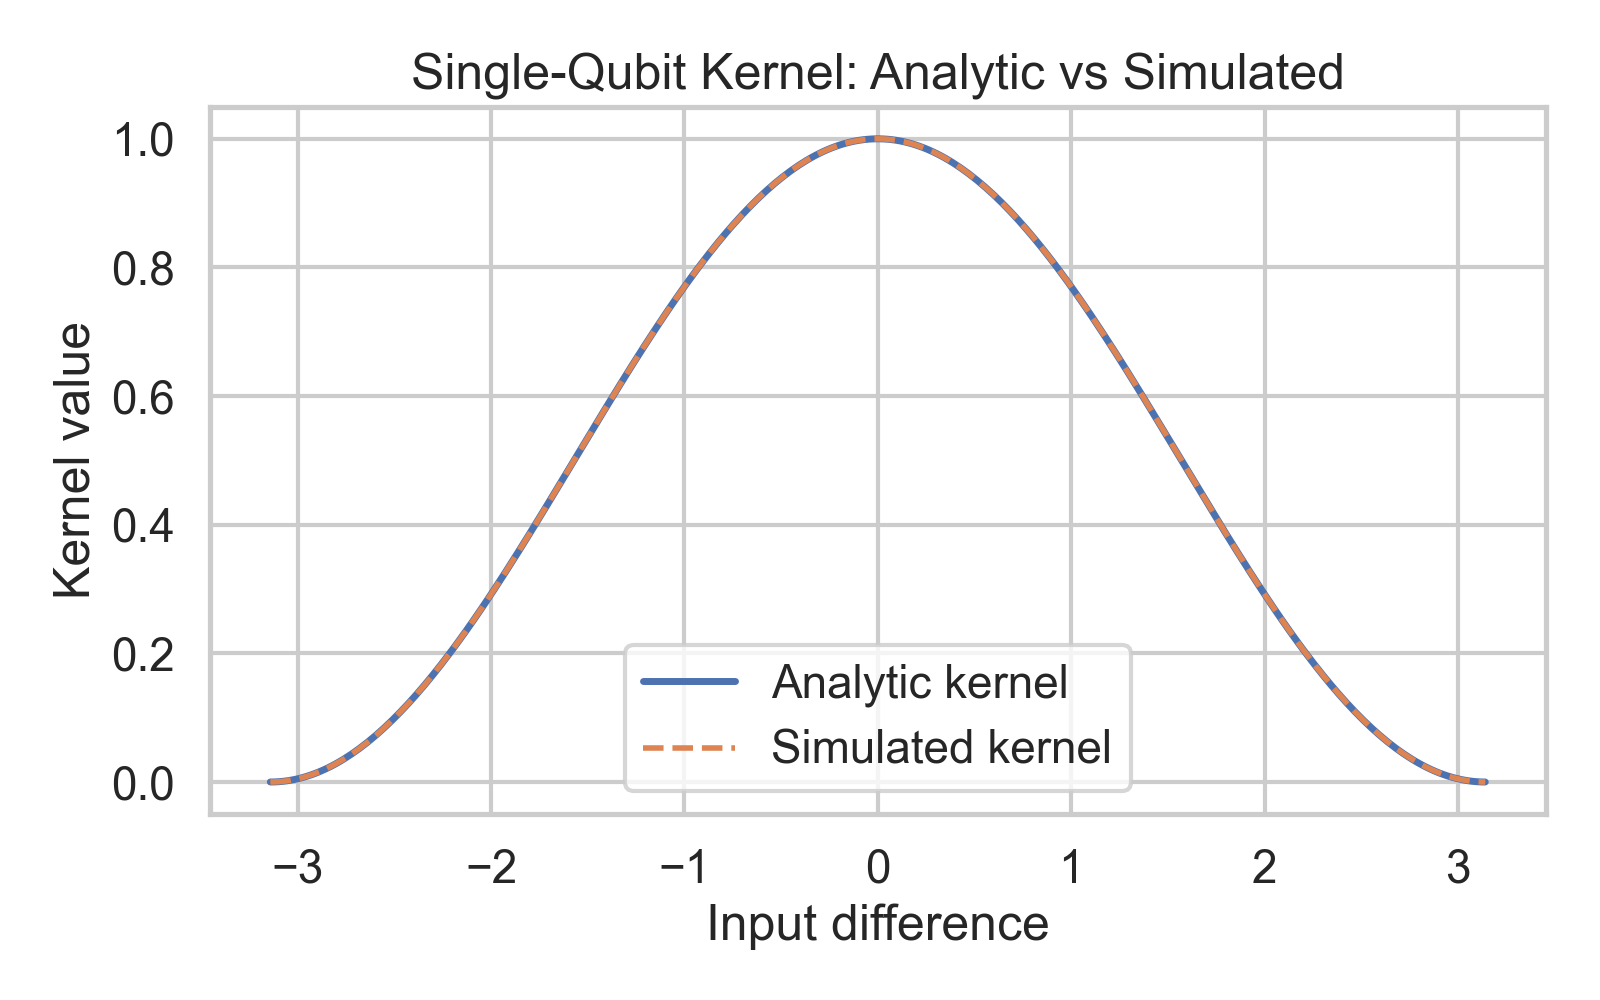
\includegraphics[width=0.72\textwidth]{analytic_vs_simulated_kernel.png}
\caption{Analytic and simulated one-qubit kernel values plotted against input difference. The horizontal axis is $x-x'$ and the vertical axis is the kernel value. The simulated statevector result lies on top of the exact expression $K(x,x')=\cos^2((x-x')/2)$, confirming the derivation. This figure was generated by the code accompanying this report.}
\label{fig:analyticcompare}
\end{figure}

\subsection{Two-qubit similarity structure}

Figure~\ref{fig:twoqubitheatmap} shows the kernel matrix for the two-qubit map on the full moon dataset after feature scaling. Compared with the single-qubit case, the structure is less obviously translation invariant and reflects both the nonlinear embedding and the ordering of samples in the dataset. The visible diagonal and repeated off-diagonal texture indicate that the circuit organizes pairwise similarities in a way that is not captured by ordinary Euclidean distance in the raw input plane. This is the concrete sense in which the quantum circuit acts as a nontrivial embedding.

\begin{figure}[H]
\centering
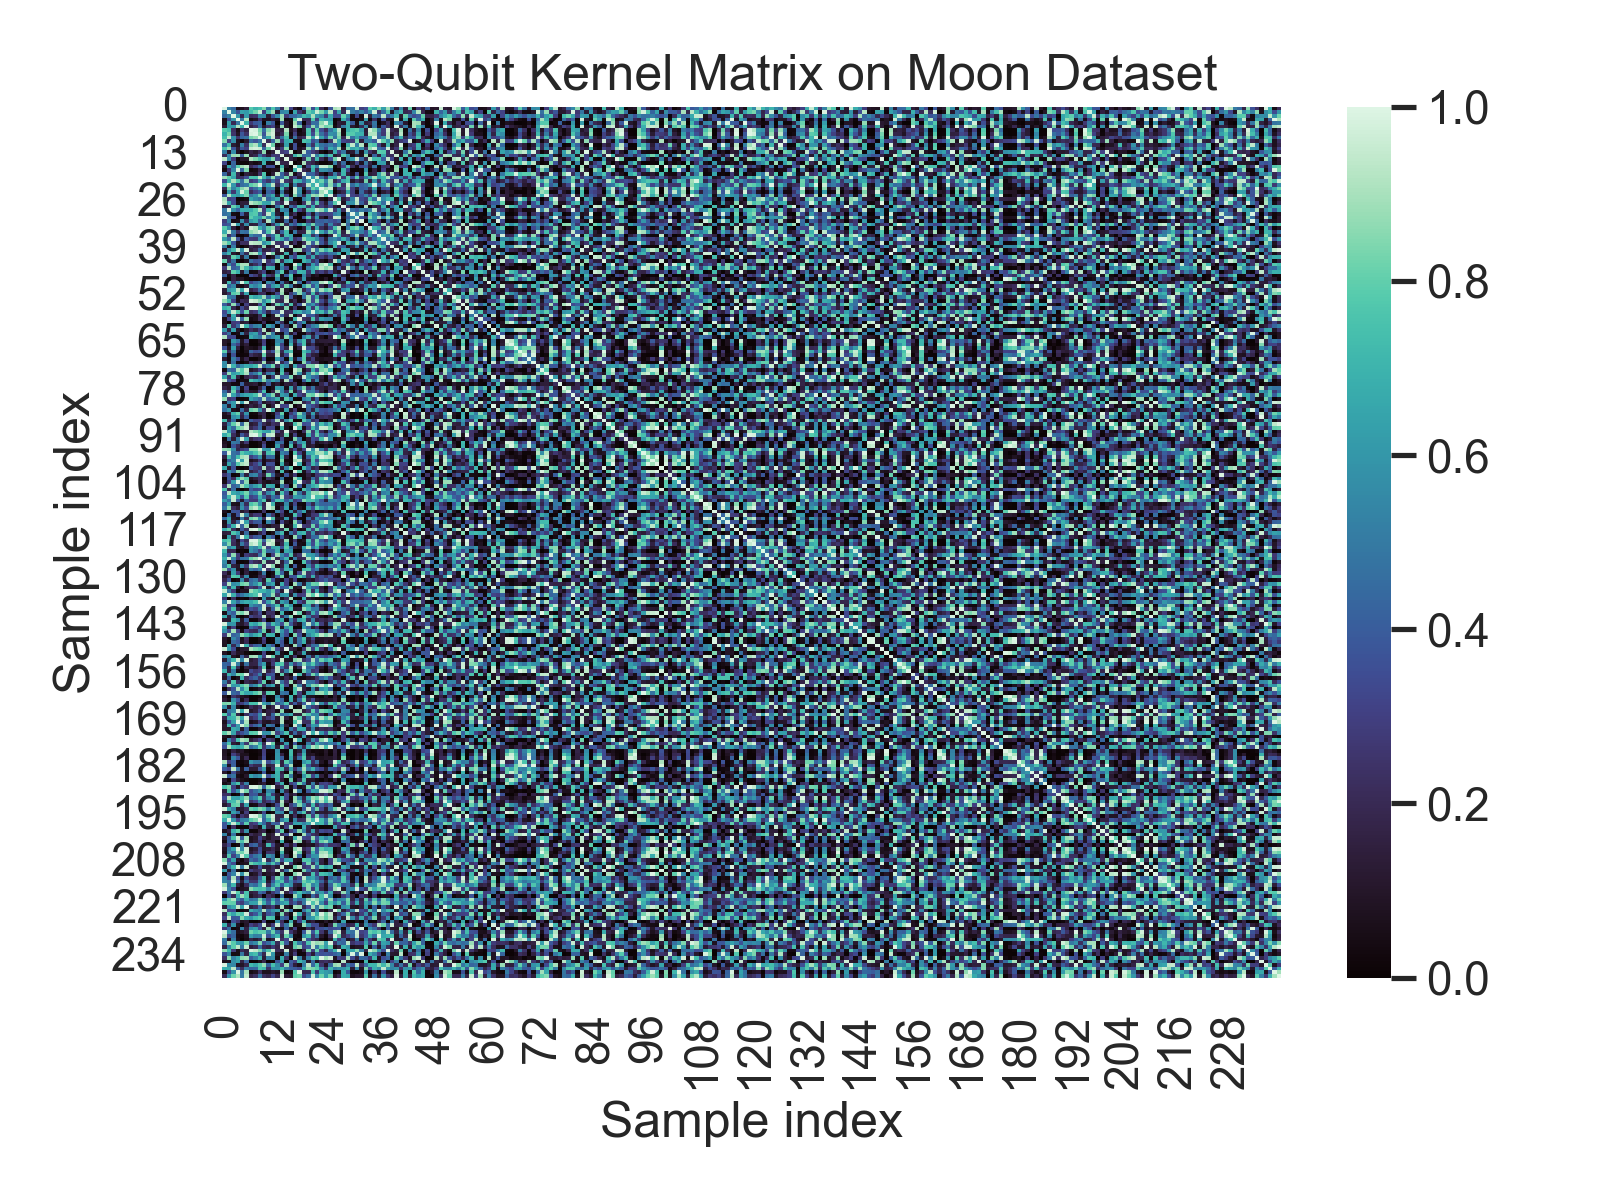
\includegraphics[width=0.72\textwidth]{two_qubit_kernel_heatmap.png}
\caption{Kernel matrix for the two-qubit entangling feature map evaluated on the full moon dataset. The horizontal and vertical axes denote sample index, and the color scale gives $K(\bm{x}_i,\bm{x}_j)$. The visible diagonal and repeated off-diagonal texture show that the circuit induces a nontrivial similarity structure across the dataset. This figure was generated by the code accompanying this report.}
\label{fig:twoqubitheatmap}
\end{figure}

\subsection{Classification performance}

The classification results are shown in Table~\ref{tab:metrics}. Logistic regression on the raw input reached a test accuracy of $0.8889$, and the degree-$3$ polynomial lift happened to yield the same value on this train-test split. The quantum-kernel SVM improved the accuracy to $0.9444$. The strongest baseline in this small experiment was the classical RBF-kernel SVM at $0.9722$.

\begin{table}[H]
\centering
\caption{Quantitative results for the classification experiment. Test accuracy is reported on the held-out $30\%$ split of the moon dataset.}
\label{tab:metrics}
\begin{tabular}{lc}
\toprule
Model & Test accuracy \\
\midrule
Raw logistic regression & 0.8889 \\
Polynomial-feature logistic regression & 0.8889 \\
Quantum-kernel SVM & 0.9444 \\
Classical RBF-kernel SVM & 0.9722 \\
\bottomrule
\end{tabular}
\end{table}

Figure~\ref{fig:decisionboundaries} compares the decision regions learned by three of the models. The raw logistic-regression boundary is nearly linear in the scaled input space and therefore cannot track the curved class structure particularly well. The polynomial model introduces some curvature but remains limited. By contrast, the quantum kernel creates a more flexible nonlinear separation in terms of similarity to the training states. The improvement in accuracy is therefore consistent with what one visually expects from the decision surfaces.

\begin{figure}[H]
\centering
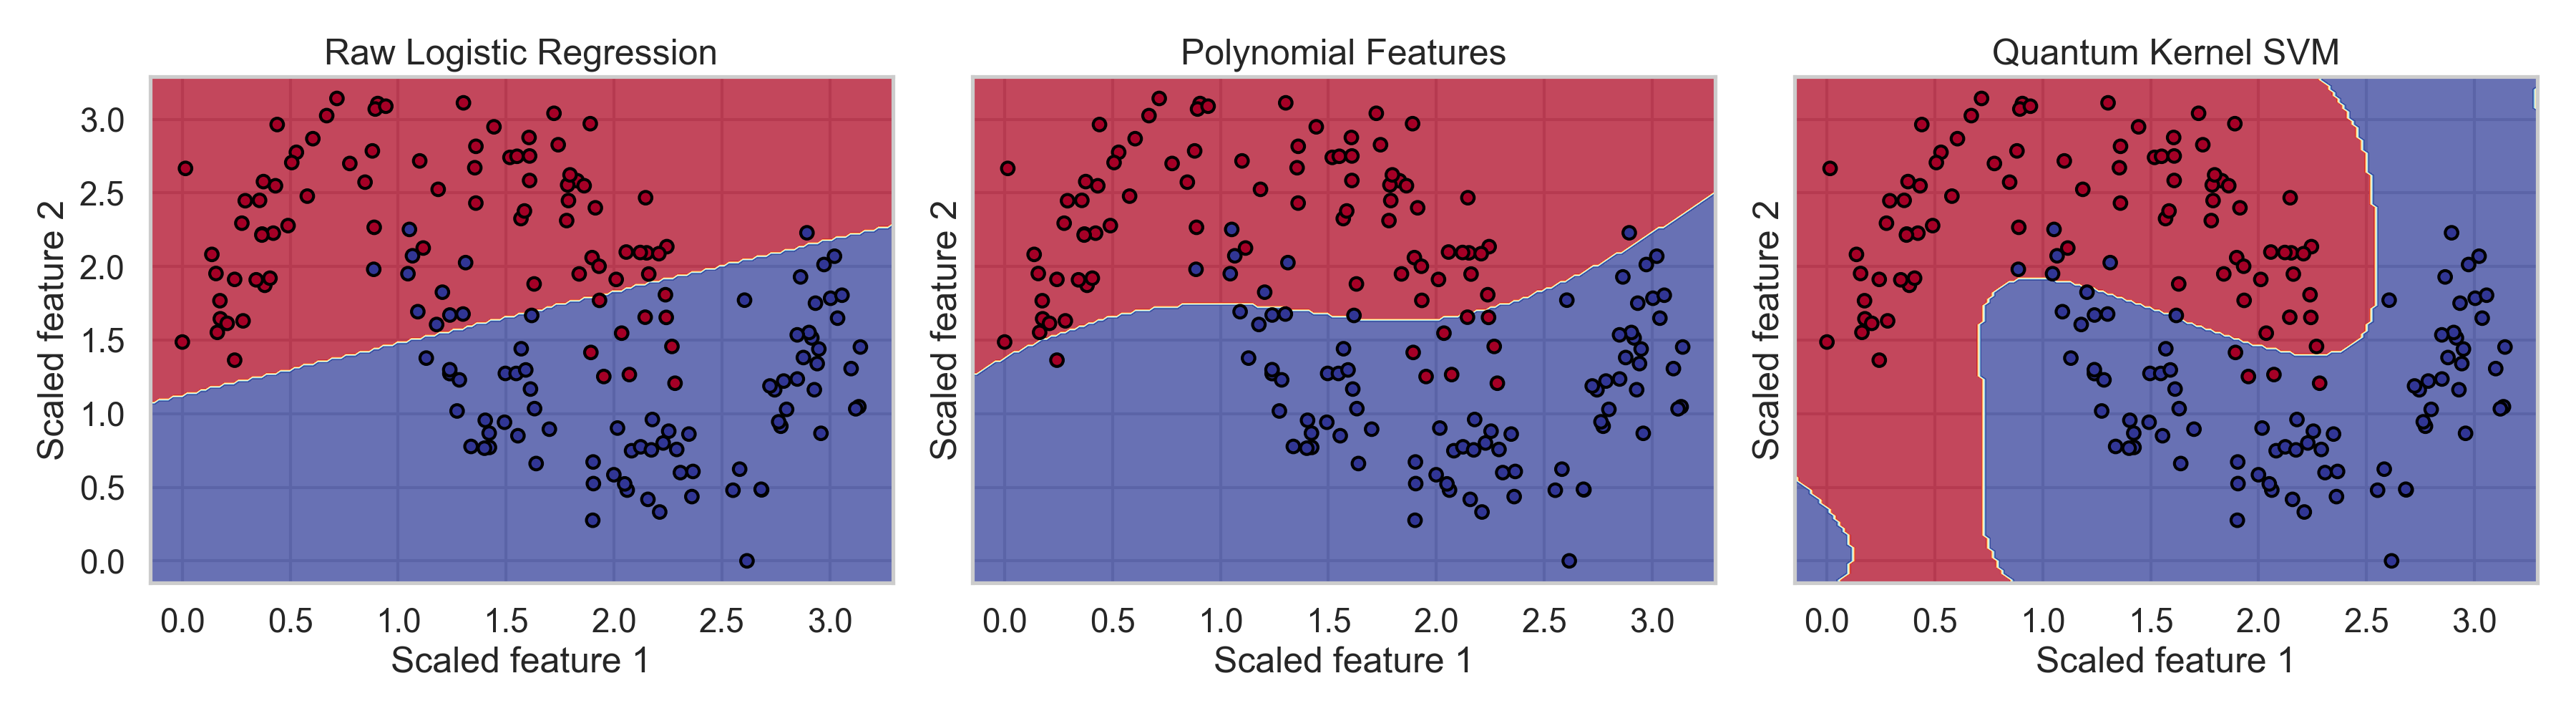
\includegraphics[width=\textwidth]{classification_comparison.png}
\caption{Decision-boundary comparison on the moon dataset. The horizontal and vertical axes are the two scaled input features, each rescaled to the interval $[0,\pi]$. From left to right the panels show logistic regression on raw inputs, logistic regression with degree-$3$ polynomial features, and an SVM using the two-qubit quantum kernel. The quantum-kernel model better follows the curved class geometry than the raw linear model. This figure was generated by the code accompanying this report.}
\label{fig:decisionboundaries}
\end{figure}

These results support the main claim of the project. The quantum feature map does behave as a useful nonlinear embedding, in the sense that it induces a similarity measure that improves performance relative to a raw linear baseline. At the same time, the experiment makes clear that this is not evidence of quantum superiority. A standard classical RBF kernel still performs slightly better on this simple dataset. That outcome is not a weakness of the project; it is exactly what should be expected for a minimal example whose purpose is interpretability rather than competitive benchmarking.

\section{Discussion}

The most important lesson from this project is that the overlap kernel offers a precise bridge between quantum mechanics and classical similarity learning. The circuit in Eq.~\eqref{eq:featuremap} is not merely a state-preparation procedure. It is also a rule for deciding which pairs of classical inputs should be considered close once they are viewed through the geometry of Hilbert space. The one-qubit derivation makes this statement mathematically explicit, while the two-qubit classification experiment shows that the changed similarity structure can have observable consequences for learning.

Several features of the construction are worth emphasizing. First, the model is modular. The quantum part chooses the representation, but the optimization is still performed by a classical SVM. Second, the overlap kernel is easy to visualize, which makes it a good teaching example. Third, the expressivity of the kernel can be increased in more than one way, for example by adding qubits, by increasing circuit depth, or by changing the entangling pattern. In this project I changed only the most basic ingredient, moving from a separable one-qubit map to a two-qubit entangling map, and even that was enough to alter the learning geometry.

There are also clear limitations. The dataset is tiny and deliberately low-dimensional. The two-qubit feature map is hand-designed rather than optimized. The kernel is computed exactly with statevectors, so no claim is made about noise robustness or sampling cost on actual hardware. Finally, because the classical baseline is already strong, the numerical gap between the quantum and classical kernels is not the interesting point. The real contribution is explanatory. The project shows concretely how a quantum state can be interpreted as an embedding and how the induced kernel enters a standard machine-learning pipeline.

One additional limitation, especially relevant for the rubric, is that the present report uses Qiskit simulation rather than IBM hardware. This was a deliberate choice. For a two-qubit pedagogical example, exact statevectors are more useful than hardware data because they isolate the geometry of the feature map without conflating it with readout noise or finite-shot fluctuations. If this project were extended into a larger study, the next natural step would be to re-run the same kernel-estimation pipeline with finite shots and compare the resulting degradation in the Gram matrix and classification accuracy.

\section{Outlook}

There are several natural directions for extending the project. A first step would be to compare multiple encodings systematically, for example replacing the present entangling map with a product map, a repeated-layer map, or one of the built-in Qiskit feature maps. This would allow one to ask which circuit ingredients most strongly affect the spectrum and geometry of the kernel matrix.

A second extension would be to move from exact statevector overlaps to finite-shot estimates using a sampler primitive or real IBM hardware. That would introduce an experimentally meaningful tradeoff between kernel quality and sampling noise. It would also connect more directly to the literature on hardware-efficient quantum kernels \cite{havlicek2019feature, qiskitkerneldocs}.

A third direction would be to analyze the kernel matrix more formally, for example through its eigenvalue spectrum or through alignment with the class labels. Such quantities could reveal why one feature map works better than another even before any classifier is trained. In a more advanced project, one could also investigate whether there are data distributions for which the chosen kernel is classically hard to approximate, which is where stronger claims about quantum advantage become relevant.

\section{Conclusion}

This project studied quantum feature maps in the simplest setting where their role is fully visible. A one-qubit rotation map yields the analytic kernel $K(x,x')=\cos^2((x-x')/2)$, and Qiskit reproduces this result to machine precision. A two-qubit entangling map generates a richer similarity structure that, when coupled to a classical SVM, improves classification accuracy relative to a linear raw-input baseline on a nonlinear toy dataset. Although the quantum kernel did not outperform a strong classical RBF kernel, the experiment succeeds in its main goal. It demonstrates in a clean, reproducible way that quantum states can be understood as embeddings and that their overlaps define usable similarity measures for machine learning.

For a PHYS 345 audience, this is a useful way to think about quantum machine learning. The point is not that a tiny quantum circuit magically solves classification problems better than classical methods. The point is that quantum mechanics gives a principled and geometrically meaningful way to construct feature spaces. Once that viewpoint is clear, more sophisticated quantum-kernel proposals become much easier to understand.

\section*{Reproducibility Statement}

All numerical values, parameter choices, and figures in this report are reproducible from the accompanying code repository. The one-qubit experiment uses $60$ points uniformly spaced in $[0,2\pi]$. The two-qubit classification experiment uses the \texttt{make\_moons} dataset with $240$ samples, noise level $0.16$, random seed $7$, a $70/30$ train-test split, and feature scaling to $[0,\pi]$. The two-qubit entangling scale is $\lambda=1.5$. The code is implemented in Qiskit and executed through the script \texttt{scripts/run\_experiment.py}, which regenerates the figures and writes the metrics to \texttt{results/metrics.json}. The full source code is intended to accompany this report as part of the submitted project materials.

If compiled in Overleaf using the included \texttt{main.tex}, \texttt{references.bib}, and the generated figure files from the \texttt{results/} directory, the reader should be able to trace every equation, figure, parameter choice, and numerical output back to the underlying source code. This is intended to satisfy the reproducibility standard stated in the PHYS 345 rubric.

\bibliographystyle{unsrt}
\bibliography{references}

\end{document}
